\RequirePackage[OT1]{fontenc}
\documentclass[conference]{IEEEtran}
\usepackage{cite}
\usepackage{amsmath,amssymb,amsfonts}
\usepackage{algorithmic}
\usepackage{textcomp}
\usepackage{graphicx, xcolor}
\usepackage{float}
\usepackage{tikz-cd}
\usepackage{lipsum}
\usepackage{hyperref, cleveref}

%--------------------------------------------------------------------------------
% Custom commands
%--------------------------------------------------------------------------------
\newcommand{\warn}[1]{\textbf{\color{red}#1}}
\newcommand{\R}{\mathbb{R}}
\DeclareMathOperator*{\argmin}{arg\,min}
\DeclareMathOperator*{\argmax}{arg\,max}

\begin{document}

%--------------------------------------------------------------------------------
% Title
%--------------------------------------------------------------------------------
\title{Homological Regularization for Autoencoders}
\author{Braden Hoagland \and Jerry Liu \and Michael Montelli}
\maketitle

%--------------------------------------------------------------------------------
% Abstract
%--------------------------------------------------------------------------------
\begin{abstract}
	Autoencoders, common generative models that learn latent representations of training data, suffer from irregular latent spaces that make generating new data difficult. Current methods for regularizing the latent space resolve this issue, but also reduce the quality of the learned embeddings by introducing stochasticity. To address this issue without affecting the autoencoder's embedding quality, we introduce a regularization penalty based on the 0-dimensional persistent homology of the learned embeddings. We show that autoencoders with this topological regularization exhibit similar generative ability to that of existing methods while maintaining deterministic learned embeddings.
\end{abstract}

%--------------------------------------------------------------------------------
% Introduction
%--------------------------------------------------------------------------------
\section{Introduction}

Generative models are a means of producing data that is qualitatively similar to some collection of training data, usually by sampling noise and transforming it. More formally, if we have a collection of $n$-dimensional points $\hat{X}$, we then can treat this as a discrete, unbiased sample of a manifold $X$ embedded in $\R^{n}$. The goal of a generative model is then to create unseen points of $X$ using only $\hat{X}$ as a reference.

A common strategy is to suppose that $X$ can be reasonably compressed into a simpler, lower-dimensional latent space $L$. If we can learn a map $L\to X$ that reconstructs $\hat{X}$ from points in $L$, and if $L$ is a simple enough space, then it should be straightforward to sample points randomly from $L$ and pass them through our reconstruction map to create unseen points in $X$.

Of course, since $X$ is in general unknown and incapable of being losslessly embedded into a lower-dimensional space, this process can only be completed approximately. One such approximation is the autoencoder, which learns representations in $L$ of points in $\hat{X}$ and then uses these representations to learn a reconstruction map $L\to X$. We will detail how autoencoders are structured and trained in \Cref{ae-summary} after introducing the general machine learning and topological concepts utilized in this paper.

%-------------------
% Deep Neural Network Training
%-------------------
\subsection{Deep Neural Network Training}

Neural networks are powerful function approximators that are frequently used in the creation of generative models. Suppose we have data $\hat{X}$ and wish to approximate a function $f:X\to Y$. If we define a differentiable map $\Delta:Y \times Y \to \R$ that is minimized if and only if both inputs are identical, then we can attempt to fit a neural network $\hat{f}$ to $f$ by minimizing
\begin{equation}
	\mathbb{E}_{x \in X}\left[ \Delta(\hat{f}(x),f(x)) \right] \approx \frac{1}{|\hat{X}|} \sum_{x\in \hat{X}} \Delta(\hat{f}(x),f(x)).
\end{equation}
To perform this minimization, we can calculate the gradient of this expression with respect to the parameters composing the neural network, then take small steps in the direction of the negative gradient. This process, stochastic gradient descent, converges almost surely to a local minimum under some moderate assumptions\cite{sgd-conv}. Although this minimum theoretically need not be the global minimum, various heuristics make stochastic gradient descent viable for finding nearly optimal solutions\cite{adam}.

With large datasets, it might be infeasible to compute $(1)$ for all of $\hat{X}$. Instead, we can sample subsets (batches) of $\hat{X}$ and take a stochastic gradient descent step using each batch. This does not affect performance in practice, so we use it in our implementations of the various algorithms in this paper. From now on, we will treat neural networks as black box function approximators, specifying only the $\Delta$ maps used during gradient descent.

%-------------------
% Persistent Homology
%-------------------
\subsection{Persistent Homology}

To capture homological properties of a point cloud, one can generate a simplicial complex from that point cloud and then compute the homology groups of that complex. One such simplicial complex generated from a point cloud is the Vietoris-Rips complex: if $\varepsilon \geq 0$ is a fixed constant and $\hat{X}$ is a set of points, we can define $\mathcal{R}_{\varepsilon}(\hat{X})$ to be the simplicial complex in which an $n$-simplex with vertices $x_0, \dots, x_{n}$ is present in the complex if and only if ${\Vert{x_i-x_j}\Vert} \leq \varepsilon$ for all $0 \leq i,j \leq n$.

Varying $\varepsilon$, we can track how the rank of the $n$-th homology group changes, giving the $n$-th dimensional persistence module of the complex. Every persistence module can be uniquely decomposed into a direct sums of interval modules, giving a set of birth-death pairs $\left\{ (b_i, d_i) \right\}_{i}$. Informally, these pairs represent when $n$-dimensional holes in the complex appear and are filled.

In this paper, we will be primarily concerned with the 0-th dimensional persistent homology. In this case, the rank of $H_{0}(\mathcal{R}_{\varepsilon}(\hat{X}))$ can be interpreted as the number of connected components of $\mathcal{R}_{\varepsilon}(\hat{X})$. A critical observation is that larger 0-dimensional death times correspond to $\text{rank } H_{0}(\mathcal{R}_{\varepsilon}(\hat{X}))$ decreasing at larger $\varepsilon$, which itself corresponds to data that is more spread out.

%-------------------
% Autoencoders
%-------------------
\subsection{Autoencoders}
\label{ae-summary}

An autoencoder is a model composed of two maps
\[
	\begin{tikzcd}
		X \rar{\mathcal{E}} & L \rar{\mathcal{D}} & X,
	\end{tikzcd}
\] 
where $X$ is some initial space containing some data $\hat{X}$ and $L$ is a latent space; usually, these are $X = \R^{n}$ and $L = \R^{m}$ for $m < n$. For any $x \in X$, its latent representation $\mathcal{E}(x)$ is an ``encoded" version of $x$ that is then ``decoded" by $\mathcal{D}$.

These maps $\mathcal{E}$ and $\mathcal{D}$ are chosen such that this encoding and decoding are as lossless as possible. We usually cannot find maps perfectly reconstructing each $x \in \hat{X}$, so we instead try to minimize the expected reconstruction difference, as in $(1)$. If $\Delta:X\times X\to \R$ is some function measuring the difference between its two inputs, we can express this as
\begin{align*}
	\argmin_{\mathcal{E}, \mathcal{D}} \; &\mathcal{L}_{\text{rec}}(X), \\
	\text{where } &\mathcal{L}_{\text{rec}}(X) := \mathbb{E}_{x \in X}\left[ \Delta(x, \mathcal{D}\mathcal{E}(x) \right].
\end{align*}

In addition to learning compressed representations of data, autoencoders can be made into generative models. If $y \sim L$, then we expect $\mathcal{D}(y)$ to be qualitatively similar to points in $X$ whose encoded representations are close to $y$. Thus in order to generate new data using an autoencoder, we need only sample points from the latent space and map them through $\mathcal{D}$.

%-------------------

\subsection{Flaws with Generative Autoencoders}
\label{ae-flaws}

Perhaps the most obvious flaw with using autoencoders as generative models is that we do not know \textit{a priori} where the encoded representations of our sample points in $X$ will be in $L$, making it difficult to sample from $L$ effectively.

To realize this problem, we trained an autoencoder with a 2-dimensional latent space ($L=\R^{2}$) on the MNIST dataset of hand-drawn digits so as to visualize the distribution of latent embeddings. MNIST images are $28 \times 28$ grayscale values, so $X = \R^{784}$, and the dataset is standard in evaluating generative models. We used a simple feed-forward architecture for both $\mathcal{E}$ and $\mathcal{D}$, each with two hidden layers of 64 nodes and using ELU activations. All outputs from the decoder were passed through a sigmoid function to ensure that only valid grayscale values were produced.

\begin{figure}[H]
	\centering
	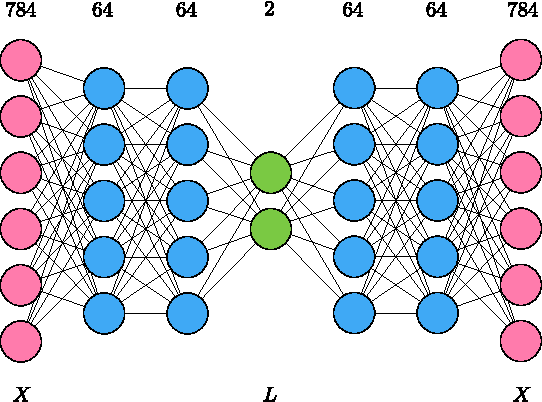
\includegraphics[scale=0.8]{fig/architecture.pdf}
	\caption{The fully connected feed-forward autoencoder architecture used throughout our experiments. The only change to this architecture in any experiment was the dimension of $L$.}
\end{figure}

To train the network, we used mean binary cross entropy as the reconstruction loss and performend batch stochastic gradient descent. Thus for a batch $B$, the total loss was
\begin{align*}
	\mathcal{L}_{\text{rec}}(B) &= - \frac{1}{|B|} \sum_{x \in B} x \log \hat{x} + (1-x) \log(1-\hat{x}), \\
	\text{where } \hat{x} &= \mathcal{D}\mathcal{E}(x).
\end{align*}

\Cref{bad-latent} shows the latent embeddings of 512 randomly sampled training images using the fully-trained autoencoder from above, where different colors represent images of different hand-drawn digits. Embeddings of the same digit are clustering together, enforcing the intuition that being close in the latent space corresponds to being close in the original space; however, the embeddings are distributed irregularly, so there is no obvious way to sample from this space with complete coverage while avoiding the indescribable regions where no embeddings lie.

\begin{figure}[H]
	\centering
	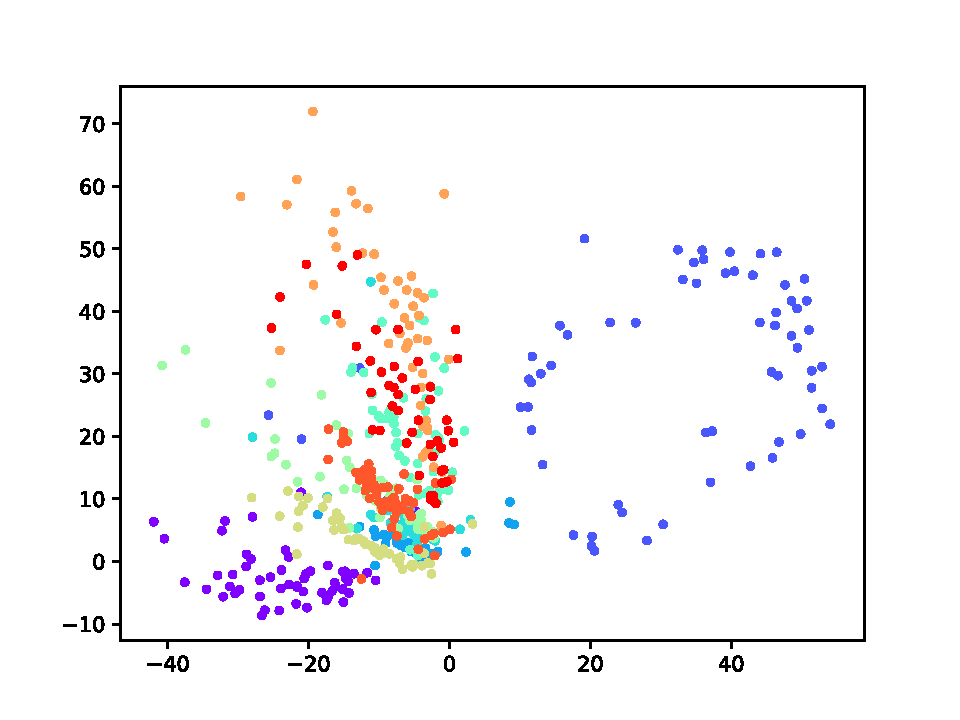
\includegraphics[scale=0.5]{fig/bad-latent.pdf}
	\caption{Latent embeddings of 512 sampled training points from the MNIST dataset after training a simple feed-forward autoencoder to convergence, where different colors represent images of different digits.}
	\label{bad-latent}
\end{figure}

%--------------------------------------------------------------------------------
% Related Work
%--------------------------------------------------------------------------------
\section{Related Work}

A common approach to addressing this sampling issue is the \textit{variational} autoencoder (VAE). Instead of $\mathcal{E}$ being a deterministic map $X\to L$, it maps points $x \in X$ to normal distributions $\mathcal{N}(\mu_{x}, \sigma^{2}_{x})$. To regularize the latent space, it minimizes the expected Kullback-Leibler divergence between the distributions output by the encoder and a standard normal distribution, which is feasible computationally since it has a closed form\cite{vae}. This forces the points in the latent space to be approximately lie in a standard normal distribution, allowing for easier sampling.

This is unsatisfying, however, as there is little reason for the embeddings to be inherently stochastic. Although useful for regularization purposes, adding noise to the latent embeddings reduces the quality of the learned representations of individual training points.

The application of a topology-based loss term to an autoencoder is not a novel idea. This same concept has been addressed by Moor et al., 2020 \cite{topo-ae}. In this paper, the authors construct a topological loss term that is shown empirically to aid in a variety of quality metrics while not having an adverse effect on the reconstruction loss. However, their loss aims to preserve topological structure of the input space in the latent representation of the autoencoder. This differs from our approach, as we try to regularize the latent space through enforcing later death times of connected components.

A recent work, \cite{birdal}, also explores the use of topological regularization for deep neural networks. Theoretical connections are made between the box dimension, a measure of model complexity, and the 0th persistent homology dimension. The authors also experiment with a loss term built upon the 0th persistence diagrams, but the complexes are computed on the model \emph{weights}, not the latent space of a generative model. Empirical experiments verify that their regularization loss term acts as a proxy for the persistent homology dimension and improves the model's generalization ability.

%--------------------------------------------------------------------------------
% Methods
%--------------------------------------------------------------------------------
\section{Methods}

We propose a topological constraint that uses the 0-dimensional persistent homology of embedded points to regularize the latent space without introducing any stochasticity. Instead of matching distributions, our constraint forces deterministic embeddings to lie approximately uniformly throughout the closed unit ball of $L$.

In particular, denote the closed unit ball of $L$ by $D_{L}$ and suppose we have a set of points $\hat{X} \subset X$. Then we seek to find $\mathcal{E}:X\to D_{L}$ and $\mathcal{D}:D_{L}\to X$ minimizing some arbitrary reconstruction loss $\mathcal{L}_{\text{rec}}$ while spreading the points $\left\{ \mathcal{E}(x) \right\}_{x \in \hat{X}}$ uniformly throughout $D_{L}$.

Approximately prohibiting embeddings from lying outside the unit ball is simple: we add a penalty term to $\mathcal{L}_{\text{rec}}$ that is 0 if a point lies within the unit ball and increases the farther a point is from the ball; however, this does not guarantee that the whole unit ball will be filled, meaning that there could still be unknown regions containing no embeddings.

To ensure that embeddings spread throughout the entirety of the unit ball, we propose maximizing the death times of the 0-dimensional persistent homology of the training points' latent embeddings. This maximization has the qualitative effect of spreading points out within the latent space: since all points in a Vietoris-Rips complex have the same fixed birth time of 0, the only way to increase death times is to move the points farther away from each other. Coupled with the penalty for leaving the unit ball, this ensures that the latent embeddings fill the unit ball without venturing outside of it.

Formally, for any batch $B$, we define a topological penalty
\[
	\mathcal{L}_{top}(B) :=  \sum_{x \in B} \max\left\{ {\Vert{x}\Vert}-1, \;0 \right\} - \sum_{d \in \dagger(B)} d,
\]
where $\dagger(B)$ is the set of 0-dimensional persistent homology death times of the Vietoris-Rips complex determined by $\mathcal{E}(B)$. The first sum penalizes points linearly based on their distance from the unit ball, and the second sum promotes large 0-dimensional death times. Thus our total loss for any batch $B$ is
\[
	\mathcal{L}_{tot}(B) := \mathcal{L}_{rec}(B) + \lambda \; \mathcal{L}_{top}(B),
\] where $\lambda$ is some hyperparameter that determines how strictly regularization is enforced. Since we expect that minimizing this modified loss will lead to latent embeddings lying in the entirety of the unit ball, we pick points uniformly from the unit ball in order to sample from the latent space.

%--------------------------------------------------------------------------------
% Implementation and Results
%--------------------------------------------------------------------------------
\section{Implementation and Results}

To test that our topological regularization had its desired effect on the latent space, we used the same setup as in \Cref{ae-flaws}. \Cref{good-latent} shows the latent embeddings of the same 512 training images after training the same number of epochs, this time with the topological regularization. These embeddings all lie roughly within the unit ball in $\R^2$ and expand to fill it entirely, meaning that sampling points from this ball gives us complete coverage of our model's learned representations while never being at risk of sampling points in regions where the model has no known behavior.

\begin{figure}[H]
	\centering
	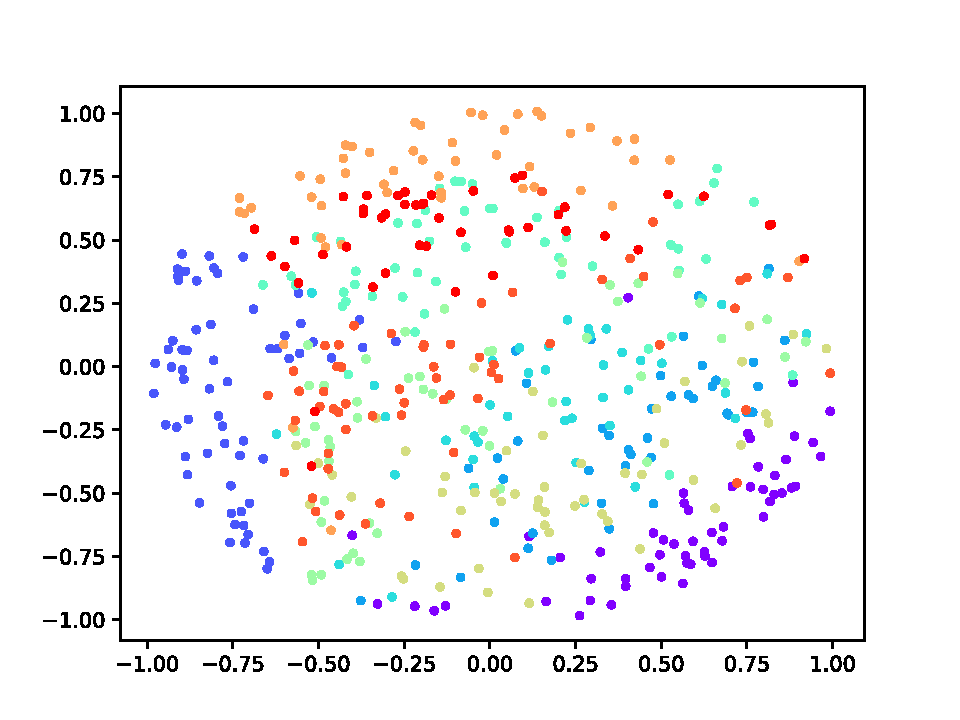
\includegraphics[scale=0.5]{fig/good-latent.pdf}
	\caption{Latent embeddings of the same 512 MNIST images from the same autoencoder architecture used for \Cref{bad-latent}, but with our topological regularization used during training.}
	\label{good-latent}
\end{figure}

To test if our regularization actually led to qualitatively better generated images, we used the same autoencoder architecture but with batch size 128. We also varied the latent space dimension among 2, 5, and 10. The standard autoencoder's latent space was sampled from by picking points from the standard Gaussian distribution, while the topologically regularized autoencoder's latent space was sampled from by picking points uniformly from the unit ball.

We trained our models using the MNIST and Fashion-MNIST datasets. While MNIST is a standard dataset for testing generative models, Fashion-MNIST contains more complicated images and thus poses a stronger challenge. \Cref{ae-2-comparison} shows example generated images from the fully trained autoencoder on MNIST with latent dimension 2 both without regularization (left) and with regularization (right). \Cref{ae-10-comparison} is the same, but the autoencoders used 10-dimensional latent spaces. Further details and results, including those for Fashion-MNIST, can be found in Appendix \hyperref[experiment-details]{A}.

For $L=\R^2$, the standard autoencoder samples points with reasonable decodings, but note the bimodality of the images: they are all either a 3, 6, or a hybrid of the two. Since the embeddings of the various digits are scattered in unknown parts of the latent space, we cannot guarantee coverage. The regularized autoencoder, on the other hand, does not suffer from this lack of coverage and produces images of a similar quality.

\begin{figure}[H]
	\centering
	\includegraphics[scale=0.4]{fig/ae-2-comparison.png}
	\caption{Generated images with $L=\R^2$. Left: without regularization. Right: with regularization.}
	\label{ae-2-comparison}
\end{figure}

\begin{figure}[H]
        \centering
        \includegraphics[scale=0.4]{fig/ae-10-comparison.png}
        \caption{Generated images with $L=\R^{10}$. Left: without regularization. Right: with regularization.}
	\label{ae-10-comparison}
\end{figure}

For $L=\R^{10}$, the irregular clusters of the standard autoencoder again prevent us from sampling effectively. Since the dataset has remained fixed while the number of latent dimensions has increased, we have increased the size of the regions in the latent space where the model has unknown behavior. It seems from \Cref{ae-10-comparison} that we have sampled from one of these regions, resulting in nonsensical images. On the contrary, the regularized autoencoder exhibits high coverage without producing uninterpretable results, and its clarity has improved over the $L=\R^2$ case, as one would expect with a higher-capacity model.

%--------------------------------------------------------------------------------
% Limitations and Discussion
%--------------------------------------------------------------------------------
\section{Limitations and Discussion}

During our experiments, there was no noticeable increase in computation time when using our topological regularization with batch size 128; however, there \textit{was} a significant increase with batch size 512 due to the increased difficulty of computing the persistent homology death times. Thus this regularization is most feasible when using small batch sizes. Further computaitonal tricks and approximations might be possible to reduce training time, but this would require further research.

Although our topological regularization was somewhat limited by batch size, it was successful in improving generative performance without sacrificing the quality of learned representations. Our regularized models were more robust with respect to the latent dimension when compared to standard autoencoders, and they generated images qualitatively similar to those of VAEs without injecting any stochasticity into the latent embeddings.

More direct relationships between our regularized autoencoders and VAEs might exist. For instance, instead of using the degree-0 total persistence $\sum_{d \in \dagger}d$ in $\mathcal{L}_{\text{top}}$, we could have used the degree-$k$ total persistence $\sum_{d \in \dagger}d^{k}$. Qualitatively, the latent embeddings would still fill all of $D_{L}$, but as $k$ increases, more would begin clustering near the origin. Determining if it is possible to approximate a standard normal distribution (and thus the latent embedding distribution of VAEs) by using variations of the total persistence like this would be an interesting topic for further research.

%-------------------
% Failed Methodologies
%-------------------
\subsection{Failed Methodologies}

Before settling on the current implementation of our topological loss term, we experimented with a variety of TDA metrics and methods. One such metric was the persistence landscape, a way to vectorize a persistence diagram. Because persistence landscapes have been shown to be both a stable and robust metric \cite{persistence-landscapes}, we thought they would encapsulate the gradual clustering of the MNIST classes throughout training so that we could use them in some capacity for a topological regularizer; however, we had difficulty determining a reasonable way of using them in this capacity and struggled with computationally efficient implementations. One thing to note is that 0-dimensional persistent homology is generally characterized by the death of each connected component, as each connected component is born at the same time. Thus, our metric does, in fact, capture the most salient features (the death times) of a persistent landscape corresponding to the 0-dimensional persistent homology.

We also considered \emph{minimizing} the 0-dimensional persistent homology death times per class while still maximizing them globally in order to promote class clustering in the latent space. Balancing these competing goals proved tricky, and our models struggled to converge with this updated objective.

%--------------------------------------------------------------------------------
% Conclusion
%--------------------------------------------------------------------------------
\section{Conclusion}
We presented a method of regularizing the latent space of autoencoders that has been shown experimentally to improve the quality of generated MNIST and Fashion-MNIST images. We utilized TDA methods, specifically persistent homology, to enforce the dispersion of points within the unit ball of the latent space while maintaining the separation of classes, leading to qualitatively realistic generated images--uniformly sampled from the latent space--that are more representative of the dataset.

As our topological loss term only requires a distance matrix between samples, it is architecture independent. So, we hope to apply our topological regularizer to more sophisticated autoencoders in the future. Furthermore, as our experimentation largely focused on the MNIST and Fashion-MNIST datasets, we hope to test our method on more complex datasets to see if the same qualitative improvements in generated images are realized. 

%--------------------------------------------------------------------------------
% Appendix A: Experiment Details
%--------------------------------------------------------------------------------
\section*{Appendix A: Experiment Details}
\label{experiment-details}

All the code used in our experiments can be found at \href{https://github.com/BCHoagland/TDA-Project}{\color{blue}github.com/bchoagland/TDA-Project}, and is based on the PyTorch and Gudhi libraries. All the collected data from our experiments can be found at \href{https://wandb.ai/bchoagland/TDA-autoencoders}{\color{blue}wandb.ai/bchoagland/TDA-autoencoders}. This includes generated images and latent embeddings (for 2-dimensional latent spaces) from every intermediate training epoch and resource allocation throughout training. Below we detail important training results that accompany those in the main body of the paper.

Throughout our experiments, we used a fixed random seed of 0 and the same feed-forward autoencoder architecture as in \Cref{ae-flaws}, with hidden layers of 64 nodes and ELU activations. We used the Adam optimization algorithm for all models with a fixed learning rate of $0.0003$. In general, we found it best to set the regularization coefficient $\lambda$ such that $\mathcal{L}_{\text{top}}$ was a small fraction of $\mathcal{L}_{\text{rec}}$. This encouraged regularization of the latent embeddings without significantly reducing the fidelity of their reconstructions. In the following experiments, we used $\lambda = 0.005$.

We also tested using separate coefficients for the disk and topological penalties. We found that the disk penalty was in general quite small compared to the topological penalty, though, so a single coefficient for both was sufficient to encourage regularization without weighting the the disk penalty too heavily.

The following two tables show generated images from autoencoders trained to convergence (in this case, 100 epochs) on the MNIST and Fashion-MNIST datasets with batch size 128 and latent dimension as listed. The left columns show generated images from standard autoencoders, and the middle columns from autoencoders trained with our topological regularization. For comparison, the right columns are from VAEs trained with the same parameters.

Note that in all cases, the standard autoencoders struggled to generate reasonable images as the latent dimension increased, and the generated images had poor coverage of the various classes in the datasets. On the other hand, the regularized autoencoders and the VAEs did not suffer from this issue at all and in fact produced images of greater clarity as the latent dimension increased. Also note that our regularization produced images of similar quality to those of the VAEs.

\begin{figure}[H]
	\centering
	\begin{tabular}{cccc}
		Latent & AE & AE+Reg & VAE \\[1mm]
		2&
		\includegraphics[width=2cm]{fig/mnist-2-false.png}&
		\includegraphics[width=2cm]{fig/mnist-2-true.png}&
		\includegraphics[width=2cm]{fig/mnist-2-vae.png}\\
		5&
		\includegraphics[width=2cm]{fig/mnist-5-false.png}&
		\includegraphics[width=2cm]{fig/mnist-5-true.png}&
                \includegraphics[width=2cm]{fig/mnist-5-vae.png}\\
		10 &
		\includegraphics[width=2cm]{fig/mnist-10-false.png}&
		\includegraphics[width=2cm]{fig/mnist-10-true.png}&
		\includegraphics[width=2cm]{fig/mnist-10-vae.png}
        \end{tabular}
\end{figure}

\begin{figure}[H]
        \centering
        \begin{tabular}{cccc}
		Latent & AE & AE+Reg & VAE \\[1mm]
		2&
                \includegraphics[width=2cm]{fig/fashion-2-false.png}&
		\includegraphics[width=2cm]{fig/fashion-2-true.png}&
                \includegraphics[width=2cm]{fig/fashion-2-vae.png}\\
                5&
                \includegraphics[width=2cm]{fig/fashion-5-false.png}&
		\includegraphics[width=2cm]{fig/fashion-5-true.png}&
                \includegraphics[width=2cm]{fig/fashion-5-vae.png}\\
                10 &
                \includegraphics[width=2cm]{fig/fashion-10-false.png}&
		\includegraphics[width=2cm]{fig/fashion-10-true.png}&
                \includegraphics[width=2cm]{fig/fashion-10-vae.png}
	\end{tabular}
\end{figure}

%-------------------
% Necessity of Topological Regularization
%-------------------
\subsection{Necessity of Topological Regularization}

It is natural to ask whether the disk penalty by itself is enough to regularize the latent space. To test this, we trained an autoencoder on the MNIST dataset using the exact same setup as in the previous experiment, except we removed the persistent homology contribution in $\mathcal{L}_{\text{top}}$. \Cref{only-disc-latent} shows how the latent embeddings for the autoencoder with $L=\R^2$, although lying entirely within $D_{L}$, do not fill the whole ball. \Cref{only-disc-images} shows how this irregularity lowers sampling quality as the dimension of $L$ increases.

\begin{figure}[H]
	\centering
	\includegraphics[scale=0.5]{fig/only-disc-latent.pdf}
	\caption{MNIST latent embeddings from an autoencoder whose only regularization was the disk penalty.}
	\label{only-disc-latent}
\end{figure}

\begin{figure}[H]
	\centering
	\includegraphics[scale=0.3]{fig/only-disc-comparison.png}
	\caption{Generated images from an autoencoder whose only regularization was the disk penalty. From left to right: $L=\R^2$, $L=\R^{5}$, and $L=\R^{10}$.}
	\label{only-disc-images}
\end{figure}

%--------------------------------------------------------------------------------
% Bibliography
%--------------------------------------------------------------------------------
\nocite{ae-survey}
\bibliographystyle{plain}
\bibliography{refs.bib}

%\nocite{thing-you-didnt-cite-but-want-in-bibliography}

\end{document}

